\documentclass[11pt,a4paper]{article}

% ---------------------------------------------------------
% Packages
% ---------------------------------------------------------
\usepackage[a4paper,margin=0.75in]{geometry}
\usepackage[T1]{fontenc}
\usepackage{lmodern}
\usepackage{microtype}
\usepackage{amsmath,amssymb}
\usepackage{graphicx}
\usepackage{booktabs}
\usepackage{xcolor}
\usepackage{tikz}
\usepackage{array}
\usepackage{hyperref}
\usepackage{fancyhdr}
\usepackage{titlesec}
\usepackage[most]{tcolorbox}
\usepackage{listings}
\usepackage{enumitem}

\usetikzlibrary{arrows.meta, positioning, shapes.geometric}

% ---------------------------------------------------------
% Color Theme
% ---------------------------------------------------------
\definecolor{IITBlue}{RGB}{0,62,116}
\definecolor{IITLightBlue}{RGB}{230,241,250}
\definecolor{CodeBg}{RGB}{248,248,248}
\definecolor{DarkGray}{RGB}{70,70,70}
\definecolor{DeepGreen}{RGB}{0,100,70}
\definecolor{BoxOrange}{RGB}{255,245,230}

% ---------------------------------------------------------
% Hyperlink Setup
% ---------------------------------------------------------
\hypersetup{
    colorlinks=true,
    linkcolor=IITBlue,
    urlcolor=IITBlue,
    citecolor=IITBlue
}

% ---------------------------------------------------------
% Header and Footer
% ---------------------------------------------------------
\pagestyle{fancy}
\fancyhf{}
\setlength{\headheight}{14pt}
\lhead{\textbf{COA Lab: Adder, Multiplier, and ALU Design}}
\rhead{\textbf{IIT Indore FDP}}
\cfoot{\thepage}

% ---------------------------------------------------------
% Section Formatting
% ---------------------------------------------------------
\titleformat{\section}
{\Large\bfseries\color{IITBlue}}
{\thesection.}
{0.5em}
{}

\titleformat{\subsection}
{\large\bfseries\color{DarkGray}}
{\thesubsection}
{0.5em}
{}

% ---------------------------------------------------------
% Code Listing Setup
% ---------------------------------------------------------
\lstdefinelanguage{Verilog}{
  morekeywords={
    module, endmodule, input, output, wire, reg, assign,
    begin, end, initial, for, integer,
    parameter, localparam, posedge, negedge
  },
  sensitive=true,
  morecomment=[l]{//},
  morecomment=[s]{/*}{*/},
  morestring=[b]"
}

\lstset{
    language=Verilog,
    basicstyle=\ttfamily\scriptsize,
    keywordstyle=\color{IITBlue}\bfseries,
    commentstyle=\color{DeepGreen},
    stringstyle=\color{red!60!black},
    backgroundcolor=\color{CodeBg},
    frame=single,
    rulecolor=\color{black!25},
    breaklines=true,
    columns=fullflexible,
    keepspaces=true,
    showstringspaces=false,
    tabsize=4,
    numbers=left,
    numberstyle=\tiny\color{gray},
    captionpos=b
}

% ---------------------------------------------------------
% Custom Boxes
% ---------------------------------------------------------
\newtcolorbox{objectivebox}{
    colback=IITLightBlue,
    colframe=IITBlue,
    arc=2mm,
    boxrule=0.8pt,
    title=\textbf{Objective}
}

\newtcolorbox{conceptbox}[1]{
    colback=white,
    colframe=IITBlue,
    arc=2mm,
    boxrule=0.8pt,
    title=\textbf{#1}
}

\newtcolorbox{exercisebox}{
    colback=BoxOrange,
    colframe=orange!80!black,
    arc=2mm,
    boxrule=0.8pt,
    title=\textbf{Lab Exercise}
}

\newtcolorbox{notebox}{
    colback=gray!8,
    colframe=gray!60,
    arc=2mm,
    boxrule=0.6pt,
    title=\textbf{Note}
}

% ---------------------------------------------------------
% Document
% ---------------------------------------------------------
\begin{document}
\pagenumbering{gobble}

% ---------------------------------------------------------
% Title Page
% ---------------------------------------------------------
\begin{titlepage}
\centering
\vspace*{1.0cm}

{\Huge \bfseries \color{IITBlue} Computer Organization and Architecture Lab\par}
\vspace{0.6cm}

{\Large \bfseries Verilog Implementation of Adders, Multipliers, and ALU Blocks for Processor Design\par}

\vspace{1.2cm}

\begin{tcolorbox}[
    colback=IITLightBlue,
    colframe=IITBlue,
    width=0.88\textwidth,
    arc=2mm,
    boxrule=1pt
]
\centering
\Large
\textbf{Faculty Development Program}\\[0.2cm]
\textbf{IIT Indore}
\end{tcolorbox}

\vspace{1.4cm}

\begin{tabular}{rl}
\textbf{Lab Duration:} & 3 Hours \\
\textbf{Material:} & Verilog HDL source files and one self-contained lab handout \\
\textbf{Prepared by:} & Mrunal Shende \\
\textbf{Department:} & Computer Science and Engineering, IIT Indore \\
\end{tabular}

\vfill

{\large \textbf{Lab Theme:} From basic arithmetic circuits to an integrated ALU datapath block}

\vspace{0.6cm}

{\large \textbf{Lab Repository:} \href{https://github.com/Mrunal321/COA-Lab}{github.com/Mrunal321/COA-Lab}}

\vspace{1cm}
\end{titlepage}
\pagenumbering{arabic}

\tableofcontents
\newpage

% ---------------------------------------------------------
\section{Aim of the Lab}

\begin{objectivebox}
The aim of this lab is to implement basic arithmetic and logic blocks used in processor datapaths using Verilog HDL. The lab begins with half adder and full adder circuits, builds a 4-bit ripple carry adder, implements a 4-bit multiplier, and finally integrates arithmetic and logical operations into a 4-bit ALU.
\end{objectivebox}

\subsection*{Learning Outcomes}

After completing this lab, participants will be able to:

\begin{itemize}[leftmargin=*]
    \item understand the role of adders, multipliers, and ALUs in processor datapaths;
    \item write Verilog modules for combinational circuits;
    \item build larger arithmetic blocks using smaller modules;
    \item understand how simple testbench inputs are applied over time;
    \item verify expected outputs using truth tables and Boolean equations.
\end{itemize}

% ---------------------------------------------------------
\section{Accessing the Lab Files}

\begin{notebox}
All Verilog source files, testbenches, and the handout are available in the lab repository:

\medskip
\centerline{\Large\textbf{\href{https://github.com/Mrunal321/COA-Lab}{github.com/Mrunal321/COA-Lab}}}

\medskip
Students should open this repository on their systems during the lab session to access the complete set of files.
\end{notebox}

% ---------------------------------------------------------
\section{Three-Hour Lab Plan}

\begin{center}
\renewcommand{\arraystretch}{1.25}
\begin{tabular}{p{3cm}p{10cm}}
\toprule
\textbf{Time} & \textbf{Activity} \\
\midrule
0:00--0:15 & Introduction to processor datapath blocks and Verilog basics \\
0:15--0:45 & Experiment 1: Half adder and full adder implementation \\
0:45--1:20 & Experiment 2: 4-bit ripple carry adder implementation \\
1:20--1:55 & Experiment 3: 4-bit multiplier implementation \\
1:55--2:35 & Experiment 4: Gate-level 4-bit ALU implementation \\
2:35--2:50 & Review of Verilog files, testbench inputs, and expected results \\
2:50--3:00 & Discussion, viva questions, and mini-assignment \\
\bottomrule
\end{tabular}
\end{center}

\begin{notebox}
This lab is designed as a single self-contained handout. The same PDF can be projected during the session and shared with participants for hands-on implementation.
\end{notebox}

\begin{conceptbox}{Suggested Presentation Flow}
\begin{enumerate}[leftmargin=*]
    \item Explain why adders, multipliers, and ALUs are basic datapath blocks.
    \item Start from Boolean expressions and then show the corresponding Verilog \texttt{assign} statements.
    \item Show the associated testbench inputs and ask participants to predict the outputs.
    \item For the ALU, first explain opcode decoding, then explain output selection using simple AND-OR logic.
\end{enumerate}
\end{conceptbox}

% ---------------------------------------------------------
\section{Background: Processor Datapath Blocks}

A processor datapath contains the hardware blocks that perform arithmetic, logic, data movement, and storage operations. In a basic processor, the ALU is one of the central datapath components. It receives operands from registers, performs an operation selected by a control signal, and produces a result.

\begin{center}
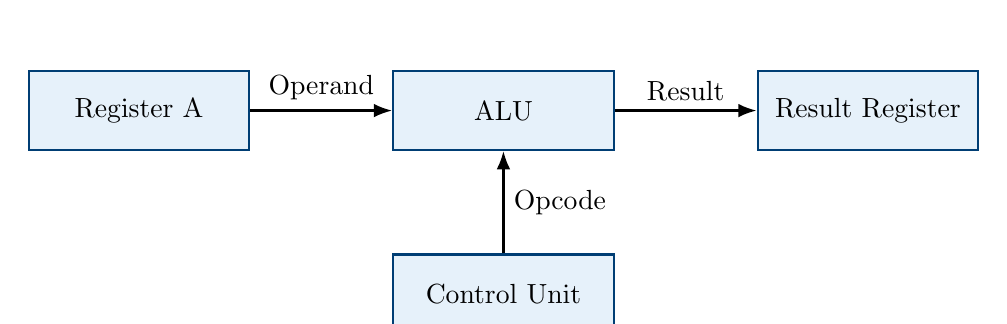
\begin{tikzpicture}[
    block/.style={rectangle, draw=IITBlue, fill=IITLightBlue, thick, minimum width=2.8cm, minimum height=1cm, align=center},
    arrow/.style={-Latex, thick}
]
\node[block] (regA) {Register A};
\node[block, right=1.8cm of regA] (alu) {ALU};
\node[block, right=1.8cm of alu] (regOut) {Result Register};
\node[block, below=1.3cm of alu] (control) {Control Unit};

\draw[arrow] (regA) -- node[above]{Operand} (alu);
\draw[arrow] (alu) -- node[above]{Result} (regOut);
\draw[arrow] (control) -- node[right]{Opcode} (alu);
\end{tikzpicture}
\end{center}

\begin{conceptbox}{Main Components Covered in This Lab}
\begin{itemize}[leftmargin=*]
    \item \textbf{Adder:} Performs binary addition.
    \item \textbf{Multiplier:} Performs binary multiplication.
    \item \textbf{ALU:} Selects and performs arithmetic or logical operations based on an opcode.
\end{itemize}
\end{conceptbox}

% ---------------------------------------------------------
\section{Verilog Basics Required for This Lab}

A Verilog design is written as a \texttt{module}. A module has input ports, output ports, internal wires, and logic statements. In this lab, design modules are written using \texttt{wire} and \texttt{assign}, so the hardware structure remains close to the Boolean equations.

\begin{lstlisting}[caption={Basic Verilog module template}]
module example_gate(
    input  wire a,
    input  wire b,
    output wire y
);

assign y = a & b;

endmodule
\end{lstlisting}

\begin{conceptbox}{Important Verilog Constructs}
\begin{itemize}[leftmargin=*]
    \item \texttt{assign}: used for continuous assignment in combinational logic.
    \item \texttt{wire}: used for connections between logic blocks.
    \item \texttt{reg}: used only in the testbench here, because testbench input values change with time.
    \item \texttt{\#10}: used in the testbench to wait for 10 ns before applying the next input.
\end{itemize}
\end{conceptbox}

% ---------------------------------------------------------
\section{Experiment 1: Half Adder and Full Adder}

\subsection{Half Adder}

A half adder adds two one-bit inputs $A$ and $B$. It produces a sum bit and a carry bit.

$$ Sum = A \oplus B = A'B + AB', \qquad Carry = A \cdot B $$

\begin{center}
\renewcommand{\arraystretch}{1.2}
\begin{tabular}{cc|cc}
\toprule
\textbf{A} & \textbf{B} & \textbf{Sum} & \textbf{Carry} \\
\midrule
0 & 0 & 0 & 0 \\
0 & 1 & 1 & 0 \\
1 & 0 & 1 & 0 \\
1 & 1 & 0 & 1 \\
\bottomrule
\end{tabular}
\end{center}

\begin{lstlisting}[caption={Verilog code for half adder}]
`timescale 1ns/1ps

module half_adder(
    input  wire a,
    input  wire b,
    output wire sum,
    output wire carry
);

assign sum   = (~a & b) | (a & ~b);
assign carry = a & b;

endmodule
\end{lstlisting}

\subsection{Full Adder}

A full adder adds three one-bit inputs: $A$, $B$, and $C_{in}$.

$$ Sum = A \oplus B \oplus C_{in} $$

$$ Sum = A'B'C_{in} + A'BC_{in}' + AB'C_{in}' + ABC_{in} $$

$$ Carry = AB + AC_{in} + BC_{in} $$

\begin{lstlisting}[caption={Verilog code for full adder}]
`timescale 1ns/1ps

module full_adder(
    input  wire a,
    input  wire b,
    input  wire cin,
    output wire sum,
    output wire cout
);

assign sum  = (~a & ~b & cin) |
              (~a &  b & ~cin) |
              ( a & ~b & ~cin) |
              ( a &  b & cin);
assign cout = (a & b) | (b & cin) | (a & cin);

endmodule
\end{lstlisting}

\subsection{Testbench for Full Adder}

\begin{lstlisting}[caption={Testbench for full adder}]
`timescale 1ns/1ps

module tb_full_adder;

reg a;
reg b;
reg cin;
wire sum;
wire cout;

full_adder uut(
    .a(a),
    .b(b),
    .cin(cin),
    .sum(sum),
    .cout(cout)
);

initial begin
    a = 0; b = 0; cin = 0; #10;
    a = 0; b = 0; cin = 1; #10;
    a = 0; b = 1; cin = 0; #10;
    a = 0; b = 1; cin = 1; #10;
    a = 1; b = 0; cin = 0; #10;
    a = 1; b = 0; cin = 1; #10;
    a = 1; b = 1; cin = 0; #10;
    a = 1; b = 1; cin = 1; #10;

    $finish;
end

endmodule
\end{lstlisting}

\begin{exercisebox}
For each input combination, use the full adder truth table to verify \texttt{sum} and \texttt{cout}.
\end{exercisebox}

% ---------------------------------------------------------
\section{Experiment 2: 4-bit Ripple Carry Adder}

A ripple carry adder is built by connecting multiple full adders in series. The carry output of one full adder becomes the carry input of the next full adder.

\begin{center}
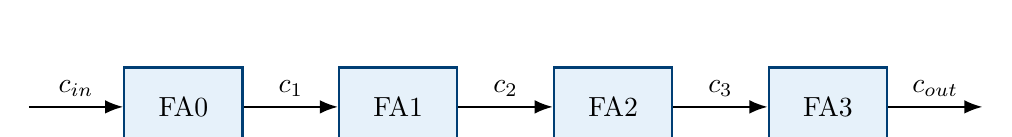
\begin{tikzpicture}[
    fa/.style={rectangle, draw=IITBlue, fill=IITLightBlue, thick, minimum width=1.5cm, minimum height=1cm, align=center},
    arrow/.style={-Latex, thick}
]
\node[fa] (fa0) {FA0};
\node[fa, right=1.2cm of fa0] (fa1) {FA1};
\node[fa, right=1.2cm of fa1] (fa2) {FA2};
\node[fa, right=1.2cm of fa2] (fa3) {FA3};

\draw[arrow] (fa0) -- node[above]{$c_1$} (fa1);
\draw[arrow] (fa1) -- node[above]{$c_2$} (fa2);
\draw[arrow] (fa2) -- node[above]{$c_3$} (fa3);
\draw[arrow] ([xshift=-1.2cm]fa0.west) -- node[above]{$c_{in}$} (fa0);
\draw[arrow] (fa3) -- node[above]{$c_{out}$} ([xshift=1.2cm]fa3.east);
\end{tikzpicture}
\end{center}

\begin{lstlisting}[caption={4-bit ripple carry adder using full adder modules}]
`timescale 1ns/1ps

module ripple_carry_adder_4bit(
    input  wire [3:0] a,
    input  wire [3:0] b,
    input  wire       cin,
    output wire [3:0] sum,
    output wire       cout
);

wire c1, c2, c3;

full_adder fa0(
    .a(a[0]),
    .b(b[0]),
    .cin(cin),
    .sum(sum[0]),
    .cout(c1)
);

full_adder fa1(
    .a(a[1]),
    .b(b[1]),
    .cin(c1),
    .sum(sum[1]),
    .cout(c2)
);

full_adder fa2(
    .a(a[2]),
    .b(b[2]),
    .cin(c2),
    .sum(sum[2]),
    .cout(c3)
);

full_adder fa3(
    .a(a[3]),
    .b(b[3]),
    .cin(c3),
    .sum(sum[3]),
    .cout(cout)
);

endmodule
\end{lstlisting}

\subsection{Testbench for 4-bit Ripple Carry Adder}

\begin{lstlisting}[caption={Testbench for 4-bit ripple carry adder}]
`timescale 1ns/1ps

module tb_ripple_carry_adder_4bit;

reg  [3:0] a;
reg  [3:0] b;
reg        cin;
wire [3:0] sum;
wire       cout;

ripple_carry_adder_4bit uut(
    .a(a),
    .b(b),
    .cin(cin),
    .sum(sum),
    .cout(cout)
);

initial begin
    a = 4'd3;  b = 4'd5; cin = 0; #10;
    a = 4'd7;  b = 4'd8; cin = 0; #10;
    a = 4'd15; b = 4'd1; cin = 0; #10;
    a = 4'd10; b = 4'd6; cin = 1; #10;

    $finish;
end

endmodule
\end{lstlisting}

\begin{conceptbox}{Discussion Point}
The delay of a ripple carry adder depends on carry propagation. The carry must travel from the least significant bit to the most significant bit. This makes the circuit simple, but not the fastest option for large bit-widths.
\end{conceptbox}

% ---------------------------------------------------------
\section{Experiment 3: 4-bit Multiplier}

A multiplier produces the product of two binary numbers. For two 4-bit inputs, the maximum value is:

$$ 15 \times 15 = 225 $$

Therefore, the product requires 8 bits.

\begin{lstlisting}[caption={4-bit combinational multiplier}]
`timescale 1ns/1ps

module multiplier_4bit(
    input  wire [3:0] a,
    input  wire [3:0] b,
    output wire [7:0] product
);

assign product = a * b;

endmodule
\end{lstlisting}

\subsection{Testbench for 4-bit Multiplier}

\begin{lstlisting}[caption={Testbench for 4-bit multiplier}]
`timescale 1ns/1ps

module tb_multiplier_4bit;

reg  [3:0] a;
reg  [3:0] b;
wire [7:0] product;

multiplier_4bit uut(
    .a(a),
    .b(b),
    .product(product)
);

initial begin
    a = 4'd3;  b = 4'd4;  #10;
    a = 4'd7;  b = 4'd2;  #10;
    a = 4'd15; b = 4'd15; #10;
    a = 4'd9;  b = 4'd6;  #10;

    $finish;
end

endmodule
\end{lstlisting}

\begin{notebox}
In this lab, the multiplication operator \texttt{*} is used to keep the implementation simple within the 3-hour session. Internally, hardware multiplication can be implemented using partial products, shift operations, and adders.
\end{notebox}

\begin{exercisebox}
As an extension, implement a 4-bit array multiplier using AND gates for partial products and adders for summation.
\end{exercisebox}

% ---------------------------------------------------------
\section{Experiment 4: 4-bit ALU Design}

An Arithmetic Logic Unit performs arithmetic and logical operations based on a control input called an opcode.

\subsection{ALU Operation Table}

\begin{center}
\renewcommand{\arraystretch}{1.25}
\begin{tabular}{ccl}
\toprule
\textbf{Opcode} & \textbf{Operation} & \textbf{Description} \\
\midrule
000 & ADD & $A + B$ \\
001 & SUB & $A - B$ \\
010 & AND & Bitwise AND \\
011 & OR  & Bitwise OR \\
100 & Student task 1 & Unimplemented in starter code \\
101 & Student task 2 & Unimplemented in starter code \\
110 & Student task 3 & Unimplemented in starter code \\
111 & Student task 4 & Unimplemented in starter code \\
\bottomrule
\end{tabular}
\end{center}

\subsection{ALU Block Diagram}

\begin{center}
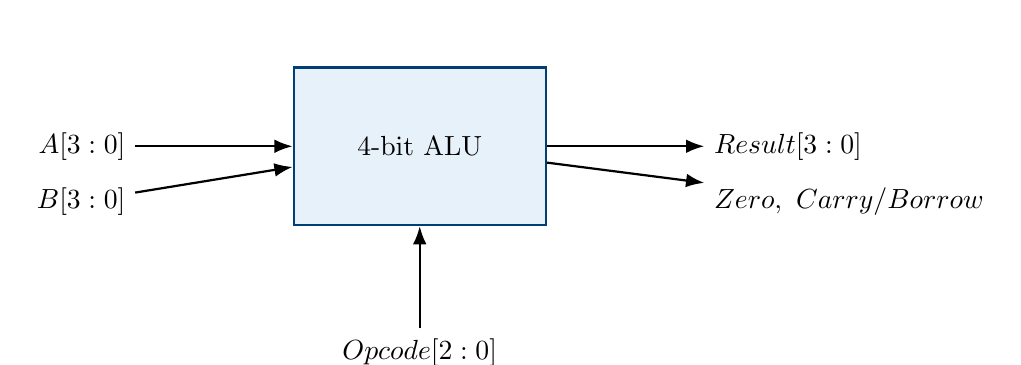
\begin{tikzpicture}[
    block/.style={rectangle, draw=IITBlue, fill=IITLightBlue, thick, minimum width=3.2cm, minimum height=2cm, align=center},
    smallblock/.style={rectangle, draw=gray, fill=gray!10, thick, minimum width=2.4cm, minimum height=0.8cm, align=center},
    arrow/.style={-Latex, thick}
]
\node[block] (alu) {4-bit ALU};
\node[left=2cm of alu] (a) {$A[3:0]$};
\node[left=2cm of alu, yshift=-0.7cm] (b) {$B[3:0]$};
\node[below=1.3cm of alu] (op) {$Opcode[2:0]$};
\node[right=2cm of alu] (res) {$Result[3:0]$};
\node[right=2cm of alu, yshift=-0.7cm] (flags) {$Zero,\ Carry/Borrow$};

\draw[arrow] (a) -- (alu);
\draw[arrow] (b) -- (alu);
\draw[arrow] (op) -- (alu);
\draw[arrow] (alu) -- (res);
\draw[arrow] (alu) -- (flags);
\end{tikzpicture}
\end{center}

\subsection{Verilog Code for 4-bit ALU}

\begin{notebox}
This starter ALU is written using structural/dataflow Verilog. It does not use \texttt{always}, \texttt{case}, or output \texttt{reg}. The starter code implements only ADD, SUB, AND, and OR. Opcodes 100--111 are intentionally left unimplemented for the assignment task.
\end{notebox}

\begin{lstlisting}[caption={Gate-level 4-bit ALU design}]
`timescale 1ns/1ps

module alu_full_adder(
    input wire a, b, cin,
    output wire sum, cout
);

assign sum  = (~a & ~b & cin) |
              (~a &  b & ~cin) |
              ( a & ~b & ~cin) |
              ( a &  b & cin);
assign cout = (a & b) | (b & cin) | (a & cin);

endmodule

module alu_4bit(
    input  wire [3:0] a,
    input  wire [3:0] b,
    input  wire [2:0] opcode,
    output wire [3:0] result,
    output wire       carry,
    output wire       zero
);

wire op2_not, op1_not, op0_not;
wire sel_add, sel_sub, sel_and, sel_or;

wire [3:0] add_result, sub_result;
wire [3:0] and_result, or_result;

wire add_c1, add_c2, add_c3, add_cout;
wire sub_c1, sub_c2, sub_c3, sub_cout, sub_borrow;

assign op2_not = ~opcode[2];
assign op1_not = ~opcode[1];
assign op0_not = ~opcode[0];

assign sel_add = op2_not & op1_not & op0_not;
assign sel_sub = op2_not & op1_not & opcode[0];
assign sel_and = op2_not & opcode[1] & op0_not;
assign sel_or  = op2_not & opcode[1] & opcode[0];

alu_full_adder add0(a[0], b[0], 1'b0, add_result[0], add_c1);
alu_full_adder add1(a[1], b[1], add_c1, add_result[1], add_c2);
alu_full_adder add2(a[2], b[2], add_c2, add_result[2], add_c3);
alu_full_adder add3(a[3], b[3], add_c3, add_result[3], add_cout);

alu_full_adder sub0(a[0], ~b[0], 1'b1, sub_result[0], sub_c1);
alu_full_adder sub1(a[1], ~b[1], sub_c1, sub_result[1], sub_c2);
alu_full_adder sub2(a[2], ~b[2], sub_c2, sub_result[2], sub_c3);
alu_full_adder sub3(a[3], ~b[3], sub_c3, sub_result[3], sub_cout);

assign sub_borrow = ~sub_cout;

assign and_result = a & b;
assign or_result  = a | b;

assign result = ({4{sel_add}} & add_result) |
                ({4{sel_sub}} & sub_result) |
                ({4{sel_and}} & and_result) |
                ({4{sel_or}}  & or_result);

assign carry = (sel_add & add_cout) |
               (sel_sub & sub_borrow);

assign zero = ~(result[0] | result[1] | result[2] | result[3]);

endmodule
\end{lstlisting}

\subsection{Testbench for 4-bit ALU}

\begin{lstlisting}[caption={Testbench for 4-bit ALU}]
`timescale 1ns/1ps

module tb_alu_4bit;

reg  [3:0] a;
reg  [3:0] b;
reg  [2:0] opcode;
wire [3:0] result;
wire       carry;
wire       zero;

alu_4bit uut(
    .a(a),
    .b(b),
    .opcode(opcode),
    .result(result),
    .carry(carry),
    .zero(zero)
);

initial begin
    a = 4'd7; b = 4'd3;

    opcode = 3'b000; #10;
    opcode = 3'b001; #10;
    opcode = 3'b010; #10;
    opcode = 3'b011; #10;

    a = 4'd15; b = 4'd1;
    opcode = 3'b000; #10;

    $finish;
end

endmodule
\end{lstlisting}

\begin{conceptbox}{Discussion Point}
The ALU uses the opcode to select one operation from multiple arithmetic and logic operations. In an actual processor, the opcode is generated by the control unit after decoding the instruction.
\end{conceptbox}

% ---------------------------------------------------------
\section{Files Provided for the Lab}

Each experiment has a Verilog design file and a small associated testbench file. The testbench only applies input values over time. It does not use display tables or tool-specific commands.

\begin{itemize}[leftmargin=*]
    \item \textbf{Half adder and full adder:} \texttt{half\_adder.v}, \texttt{full\_adder.v}, \texttt{tb\_half\_adder.v}, \texttt{tb\_full\_adder.v}
    \item \textbf{Ripple carry adder:} \texttt{full\_adder.v}, \texttt{ripple\_carry\_adder\_4bit.v}
    
    Testbench: \texttt{tb\_ripple\_carry\_adder\_4bit.v}
    \item \textbf{Multiplier:} \texttt{multiplier\_4bit.v}, \texttt{tb\_multiplier\_4bit.v}
    \item \textbf{ALU:} \texttt{alu\_4bit.v}, \texttt{tb\_alu\_4bit.v}
\end{itemize}

% ---------------------------------------------------------
\section{Common Debugging Issues}

\begin{center}
\renewcommand{\arraystretch}{1.25}
\begin{tabular}{p{4.3cm}p{8.5cm}}
\toprule
\textbf{Issue} & \textbf{Possible Reason} \\
\midrule
Output remains unknown \texttt{x} & Input values may not be initialized in the testbench \\
Compilation error & Module name or port name mismatch \\
Wrong multiplier output & Product width may be too small \\
ALU result incorrect & Opcode mapping may be wrong \\
Carry/borrow not visible & Carry output may not be connected or displayed \\
Simulation does not stop & Missing \texttt{\$finish} statement \\
\bottomrule
\end{tabular}
\end{center}

% ---------------------------------------------------------
\section{Mini-Assignment}

\begin{exercisebox}
Complete any two of the unimplemented ALU opcode slots 100--111. You may choose from the following operations, or propose another operation to the instructor:

\begin{enumerate}[leftmargin=*]
    \item NAND
    \item NOR
    \item XOR
    \item NOT of input $A$
    \item Logical shift left or logical shift right of input $A$
\end{enumerate}
\end{exercisebox}

% ---------------------------------------------------------
\section{Viva and Discussion Questions}

\begin{enumerate}[leftmargin=*]
    \item Why is a full adder required in multi-bit addition?
    \item What is the main limitation of a ripple carry adder?
    \item Why does a 4-bit multiplier produce an 8-bit output?
    \item What is the role of opcode in an ALU?
    \item What is the difference between combinational and sequential logic?
    \item Why do we need a testbench in HDL design?
    \item How is the zero flag useful in processor design?
    \item How can the ALU be extended for a real processor datapath?
\end{enumerate}

% ---------------------------------------------------------
\section{Conclusion}

In this lab, participants implemented basic arithmetic and logic blocks used in processor datapaths. The lab started with half adder and full adder circuits, extended them to a 4-bit ripple carry adder, introduced multiplier design, and finally integrated multiple operations into a 4-bit ALU. These blocks form the foundation of arithmetic and logic execution inside a processor.

\vspace{0.5cm}

\begin{center}
\begin{tcolorbox}[
    colback=IITLightBlue,
    colframe=IITBlue,
    width=0.85\textwidth,
    arc=2mm,
    boxrule=1pt
]
\centering
\Large \textbf{End of Lab}
\end{tcolorbox}
\end{center}

\end{document}
